\documentclass{article}
\usepackage{amsmath}
\usepackage{graphicx}
\begin{document}
\title{Equations of Lines: Question 10}
\author{Ana Bhattacharjee}
\date{\today}
\maketitle{}

\begin{center}
An image of the trapezoid is shown below.
\begin{figure}
  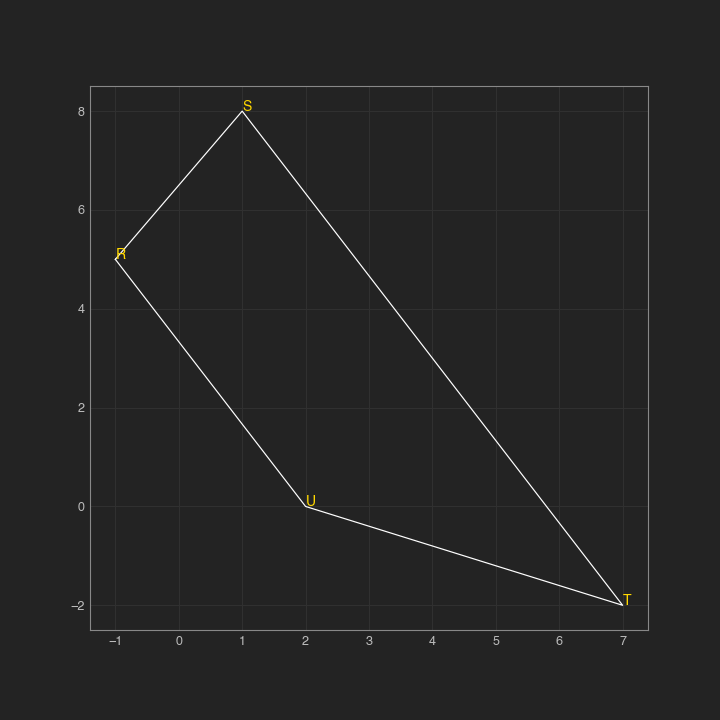
\includegraphics[width=1.1\columnwidth]{../line_eq_q10}
  \caption{Trapezoid}
\end{figure}
\par
To find the line containing the median of the trapezoid, we first need to calculate the midpoint of the longer base as the median is the line drawn from the top corner vertex tp the midpoint of the long base. The long base is ST and the corner vertex is U.
\begin{align}
S (1, 8) \\
T (7, -2) \\
M = (\frac{1 + 7}{2}, \frac{8 + (-2)}{2}) \\
M (4, 3)
\end{align}
Calculate the slope of the median line using the coordinates of M and U and substitute the slope into slope intercept form.
\begin{align}
U (2, 0) \\
\text{slope} = \frac{3 - 0 }{4 - 2} = \frac{3}{2} \\
y = mx + b \\
y = \frac{3}{2}x + b \\
3 = \frac{3}{2}4 + b \rightarrow 3 = 6 + b \rightarrow b = -3  \\
y = \frac{3}{2}x - 3
\end{align}
\end{center}

\end{document}
